\documentclass[border=3pt]{standalone}
% Preâmbulo compartilhado pelos diagramas TikZ da aula 13 (SLAM com EKF)
\usepackage[T1]{fontenc}
\usepackage[utf8]{inputenc}
\usepackage{lmodern}
\usepackage{amsmath}
\usepackage{xcolor}
\usepackage{tikz}
\usetikzlibrary{arrows.meta,angles,quotes,decorations.pathmorphing,decorations.pathreplacing,calc,
                positioning,shapes.geometric,shapes.misc,backgrounds,fit,
                math}

% Paleta (mesma dos SVGs originais)
\definecolor{dblue}{HTML}{2A5B8C}
\definecolor{dorange}{HTML}{B3541E}
\definecolor{dgreen}{HTML}{4A7C59}
\definecolor{dred}{HTML}{9C4B4B}
\definecolor{dcream}{HTML}{F4F1EA}
\definecolor{dshade}{HTML}{DDD7C9}

% Função gaussiana (não normalizada por padrão de escala visual)
\pgfmathdeclarefunction{gauss}{3}{%
  \pgfmathparse{1/(#3*sqrt(2*pi))*exp(-((#1-#2)^2)/(2*#3^2))}%
}

% Estilos comuns (prefixo d... para não colidir com chaves internas do pgf)
\tikzset{
  >={Stealth[length=2mm]},
  dguide/.style={gray!55, dashed, line width=0.4pt},
  daxis/.style={gray!60, line width=0.7pt, ->},
  dbody/.style={fill=black!3, draw=black!80, line width=1pt},
  dacc/.style={draw=dblue, line width=1pt},
  dlbl/.style={black!55, font=\small},
  dsub/.style={black!45, font=\footnotesize},
  dstate/.style={circle, draw=black!80, fill=dcream, line width=1pt,
                 minimum size=17mm, font=\large, inner sep=1pt},
  dobs/.style={circle, draw=black!80, fill=dshade, line width=1pt,
               minimum size=14mm, font=\large, inner sep=1pt},
  dbox/.style={rounded corners=2pt, draw=black!80, fill=dcream, line width=1pt,
               align=center, inner sep=6pt},
  dop/.style={circle, draw=black!80, fill=white, line width=1pt,
              minimum size=6mm, inner sep=0pt, font=\small},
  dtrans/.style={->, dblue, line width=1pt},
  dmeas/.style={->, dorange, line width=1pt},
  dcurve/.style={line width=1pt, dblue},
  dcurveb/.style={line width=1.4pt, dorange},
}

\begin{document}
\hyphenpenalty=10000 \exhyphenpenalty=10000 \tolerance=9999 \emergencystretch=3em
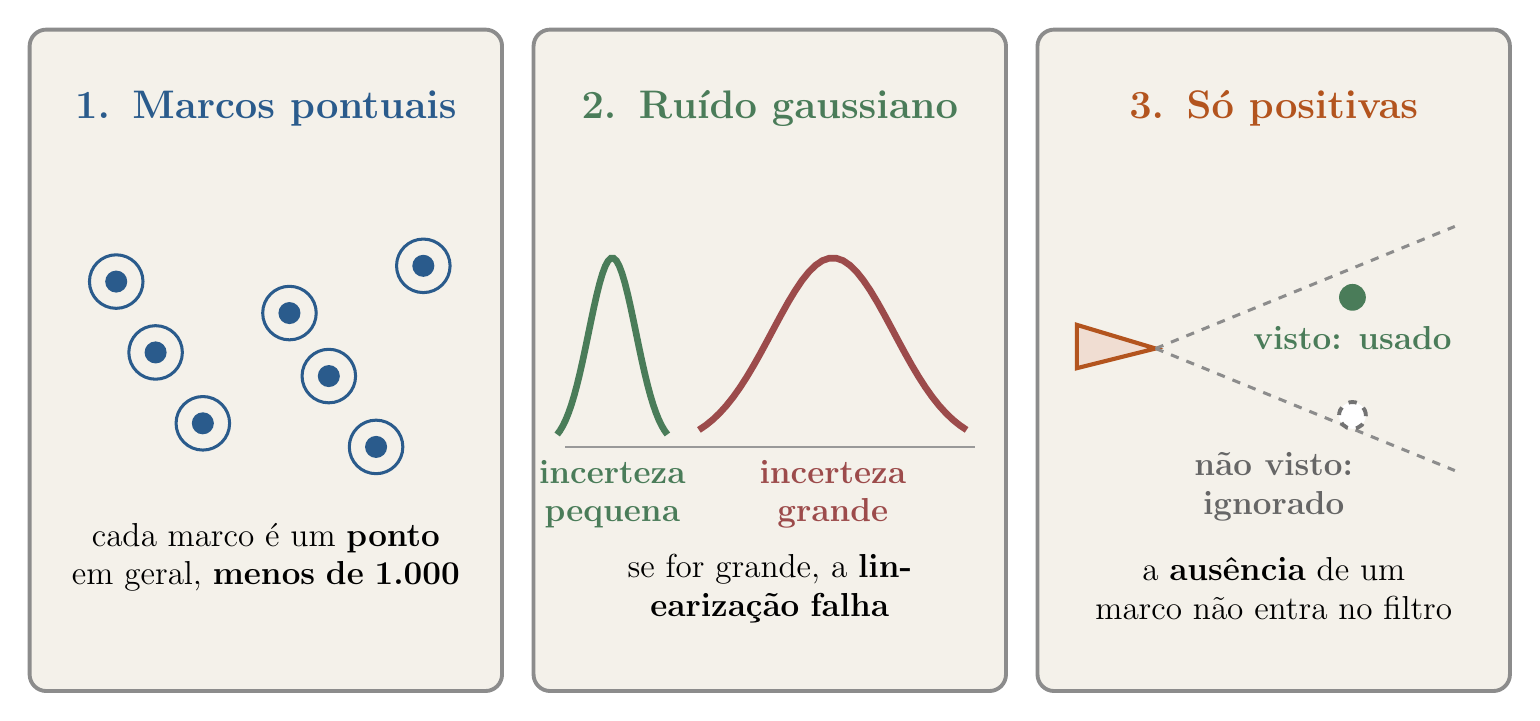
\begin{tikzpicture}[x=1cm,y=1cm]
\tikzset{c/.style={draw=black!45, line width=1.4pt, rounded corners=6pt, fill=dcream}}
\draw[c] (0.2,0.2) rectangle (6.2,8.6); \draw[c] (6.6,0.2) rectangle (12.6,8.6); \draw[c] (13.0,0.2) rectangle (19.0,8.6);
\node[font=\Large\bfseries, dblue, text width=5.6cm, align=center] at (3.2,7.6) {1. Marcos pontuais};
\node[font=\Large\bfseries, dgreen, text width=5.6cm, align=center] at (9.6,7.6) {2. Ruído gaussiano};
\node[font=\Large\bfseries, dorange, text width=5.6cm, align=center] at (16.0,7.6) {3. Só positivas};
% 1: poucos pontos
\foreach \x/\y in {1.3/5.4,2.4/3.6,3.5/5.0,4.6/3.3,5.2/5.6,1.8/4.5,4.0/4.2} {
  \fill[dblue] (\x,\y) circle (0.14); \draw[dblue, line width=1.1pt] (\x,\y) circle (0.34);}
\node[font=\large, text width=5.4cm, align=center] at (3.2,1.9) {cada marco é um \textbf{ponto}\\ em geral, \textbf{menos de 1.000}};
% 2: gaussianas
\draw[black!40, line width=1pt] (7.0,3.3) -- (12.2,3.3);
\draw[dgreen, line width=2.4pt, domain=6.9:8.3, samples=40] plot (\x, {3.3+2.4*exp(-((\x-7.6)^2)/(2*0.09))});
\draw[dred, line width=2.4pt, domain=8.7:12.1, samples=40] plot (\x, {3.3+2.4*exp(-((\x-10.4)^2)/(2*0.6))});
\node[font=\large\bfseries, dgreen, text width=2.2cm, align=center] at (7.6,2.7) {incerteza\\ pequena};
\node[font=\large\bfseries, dred, text width=3cm, align=center] at (10.4,2.7) {incerteza\\ grande};
\node[font=\large, text width=5.4cm, align=center] at (9.6,1.5) {se for grande, a \textbf{linearização falha}};
% 3: só o que foi visto
\draw[dorange, fill=dorange!20, line width=1.5pt] (13.5,4.3) -- (14.5,4.55) -- (13.5,4.85) -- cycle;
\draw[black!45, dashed, line width=1.1pt] (14.5,4.55) -- (18.3,6.1); \draw[black!45, dashed, line width=1.1pt] (14.5,4.55) -- (18.3,3.0);
\fill[dgreen] (17.0,5.2) circle (0.17); \node[font=\large\bfseries, dgreen, anchor=north] at (17.0,4.95) {visto: usado};
\draw[black!55, dashed, line width=1.4pt, fill=white] (17.0,3.7) circle (0.17); \node[font=\large\bfseries, black!60, anchor=north, text width=4cm, align=center] at (16.0,3.35) {não visto: ignorado};
\node[font=\large, text width=5.4cm, align=center] at (16.0,1.5) {a \textbf{ausência} de um marco não entra no filtro};
\end{tikzpicture}
\end{document}
